\chapter{Design}
\addcontentsline{toc}{chapter}{Design}

\section{Software Functionality and Architecture}
	
	We have decided to call our project ``Tagger3D''.  Since the purpose is to classify (or tag) point clouds, the name seems suitable. An optimal combination of algorithms for a bag of words pipeline is task and data specific. To find a combo of routines that yields superior performance we have to evaluate numerous algorithms. The process can be simplified; We are going to design an application that can be easily configured and extended. It should be possible to configure and choose an algorithm at run-time. Moreover, it should enable real time classification if it is to be used in any real setting.
	
	\subsection{Required functionality}	
	There are three major functions that have to be supported by the programme:
	\begin{enumerate}
	 \item train --- performs training
	 \item test --- evaluates the previously trained classifier
	 \item infer --- predicts a category of a single object
	\end{enumerate}
	
	Before any of them can be implemented, we have to identify common features. Inference and testing is very similar. The only difference is that the latter should process a whole testing dataset and compute statistics. The inference and training processes looks as follows:
	
	\begin{tabular}{p{0.5\textwidth}p{0.5\textwidth}}
		Inference:
		\begin{enumerate}
			\item RGBD image reading and preprocessing
			\item Point cloud construction
			\item Salient region identification
			\item Feature Extraction
			\item Vector Quantization
			\item Classification
		\end{enumerate} 
		&
		Training:
		\begin{enumerate}
		\item RGBD image reading and preprocessing
		\item Point cloud construction
		\item Salient region identification
		\item Feature Extraction
		\item Codebook Construction
		\item Vector Quantization
		\item Classificator training
		\end{enumerate} \\
	\end{tabular}
	
	The only differences is that training stage requires codebook construction and classifier training, whereas inference uses the classifier for prediction. If we compare training to testing it is clear that they both deal with large amounts of data. Inference is not that data-intensive and can be carried out for a single image. In order to simplify training we have decided to split the training and testing phases into several sub-routines. Such treatment let us change settings of an algorithm without the need to retrain the stages that lay before considered algorithm in the pipeline (\emph{e.g.} there is no need to extract features once more only because we have changed the dictionary size). The final application has the following operational modes, accessible from the command line:
	
	\begin{enumerate}
		\item Feature Extraction
		\item Codebook Generation
		\item Classifier Training
		\item Classifier Evaluation
		\item Inference
	\end{enumerate}
	
	In order to ensure that the application is configurable and easily extensible we used singleton and strategy design patterns and resorted to the Boost's program\_options package for configuration file parsing.
	
		\subsubsection{Input/Output operations}	
		This work is extremely data dependent. Every operation requires external data. Both training and testing a classifier consumes hundreds of images. Datasets used in this projects have different and incompatible formats. Not only an object responsible for run-time input/output operations is needed, but also a set of scripts for data preprocessing. Additionally, some serialisation method have to be supplied. The training of the classifier is far too computationally expensive to be computed every time the application starts. Once the classifier is trained, all the models should be stored for further usage. A way of saving and loading codebook and svm model is required. 
		
		\subsubsection{Configuration}		
		Every algorithm used in this work have several configuration parameters. If the parameters were to be compiled with the code, every change would require a rebuild of parts of the application. A run-time configuration functionality is essential. 
		
		\subsubsection{Interchangeability of algorithms}		
		Multitude of available algorithms makes it time consuming and computationally expensive to evaluate every available option. It should be possible to build the programme with a number of algorithms suitable for performing the same task and decide which one should be used at run-time.
		
	\subsection{Architecture}
	
	\begin{figure}[ht]
	\centering
	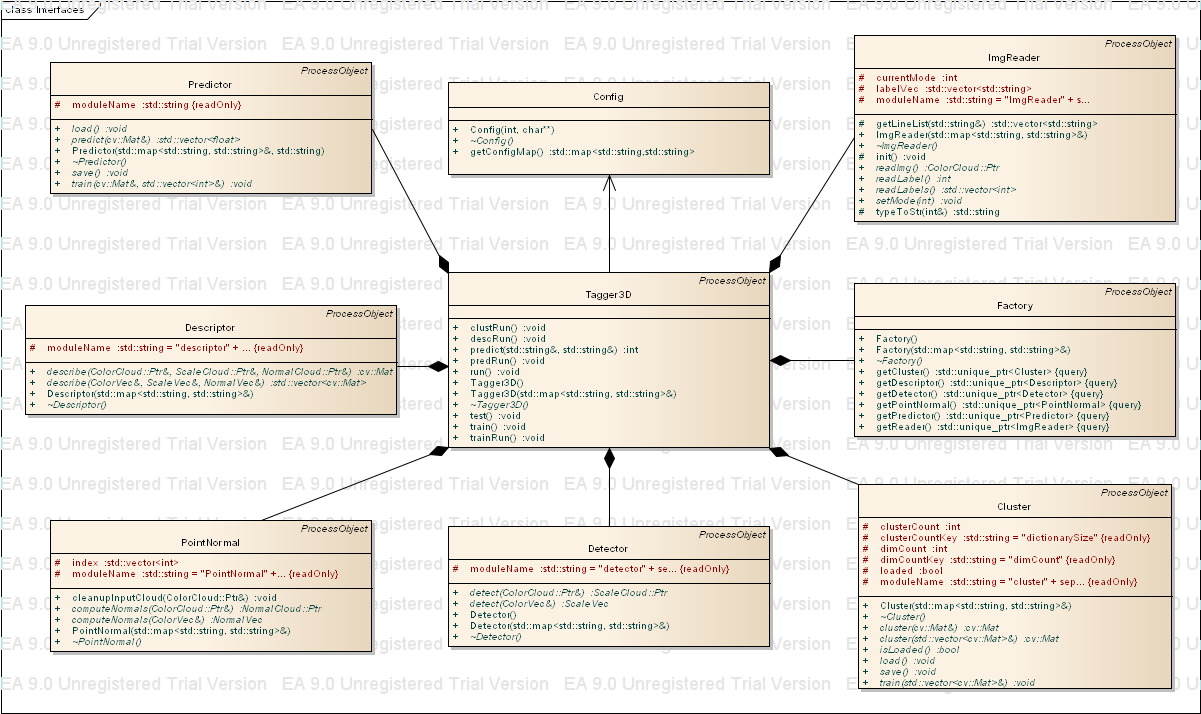
\includegraphics[width=1.0\textwidth]{figs/class}
	\caption{Tagger3D class diagram}
	\label{fig:class_diagram}
	\end{figure}
	
	C++ is one of the most efficient languages on the market. It is perfect for Object Oriented Programming (OOP) --- a paradigm that makes writing modular, flexible and extensible software easier. The excellent meta-programming tools provided by the language help to minimise the length of the hand-written code. Among OOP's best practices is to use design patterns - a set of well-known, documented and tested methods of solving certain architectural problems. Using design patterns leads to cleaner code which is easier to maintain and reuse. 
	
	\subsubsection{Configurability}
	The programme is configurable through a text file of a standard *.ini format. It should be formatted as follows:
	\begin{tabular}{c}
	 param1 = 2
	 param2 = aha
	 [section]
	 param3 = no
	\end{tabular}
	
	On top of the file there is a global section. Parameters can be accessed by their names. We can define sections but putting a section's name in brackets. the param3 can be accessed as ``section.param3''. An object ``Config'' was created for the purpose of configuration file parsing. It uses the Boost.program\_options module. Returned associative array of (parameter, value) pairs contains all parameters from a configuration file. We use a convention that if any object has to be configured by the configuration map it has to accept this map in it's constructor.
	
	\subsubsection{Strategy Design Pattern}
	
	\begin{figure}[ht]
	\centering
	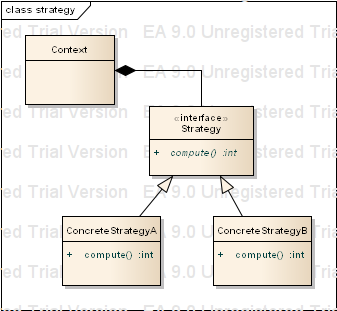
\includegraphics[width=0.5\textwidth]{figs/strategy}
	\caption{Strategy pattern}
	\label{fig:strategy}
	\end{figure}
	
	Design patterns were for the very first time by Gamma \emph{et al} in 1993 \cite{gamma1993design}. They are best practices that should be used to solve recurring problems in software design. One of the patterns is the strategy pattern. It enables implementation of multiple algorithms to handle one task. Then, a specific algorithm can be selected at run-time. It is the exact problem encountered here. It is stated that an interface should be defined for each task and multiple classes encapsulating different algorithms for handling the task should realise the interface. One modification has been done: Algorithms have often some common operations, thus an idea of an interface (a class without any implemented methods) was dropped in favour of an abstract class with some methods implemented. 
	
	The strategy pattern was used for every processing step of the pipeline so as to make it extensible. This property can be enhanced further by using a pattern of abstract factory. The idea was dropped in this case, however. The project is relatively small and the bulk of an abstract factory is beyond reason.
	
	Six parts of the pipeline are a subject of strategy pattern. The interfaces representing them are: ImgReader, PointNormal, Detector, Descriptor, Cluster, Predictor. Each of them contains pure virtual computation methods --- 'read` in case of the ImgReader or 'predict' in case of the Predictor. Additionally, they have some common methods defined --- I/O methods in Cluster or batch processing methods (such that take a vector of elements instead of a single element as an input) for the Detector and the Descriptor. Every pure virtual class have its specialisations. For instance there is the PFHDescriptor class with a Point Feature Histogram descriptor or a KMeansCluster employing kMeans clustering algorithm. The Factory class chooses specialisations of the algorithms at run-time, depending on the configuration parameters.
	
	